%!TEX program = xelatex
%!TEX root = ../thesis.tex
\chapter{Data Collecting and Modeling}\label{chap:data_collecting_modeling}
% 这部分,关于实验数据处理的描述,会比较难改
Our experimental evaluation aims to guide the GreenEyes system to analyze the current status of ambient air quality and learn to make proper predictions. If possible, we hope to design the system to take smart control actions like turning on/off the air purifier's fan.

This chapter's process shows that the raw PM data are unsuitable for direct feeding to the model. We innovatively developed a polygonization method that shows manual labeling on the IAQI levels is useful. It creates an appropriated target label function that the model can learn. Also, based on the labeling tricks, the problem that the predictions on the IAQI level will fluctuate near the thresholds is quite reduced. Furthermore, it comes from a real scenario when users interact with this machine learning product and system.

\section{Data Collecting}

We placed our four sensors in an office room located inside the Academic Building of the Hong Kong University of Science and Technology. The room is inside the academic building and has no windows. It provides a stable experimental environment for temperature and humidity. Figure \ref{fig:sensor_placement} shows the placement of these 4 sensors.

\begin{figure}[!htbp]
    \begin{center}
    \includegraphics[width=\linewidth]{fig/sensor_placement_20191125/sensor_placement.png}
    \end{center}
    \caption{Sensor placement, sensor 0 to sensor 3 locates from left to right.}
    \label{fig:sensor_placement}
\end{figure}

The sampling rate of the sensor is 1 Hz, meaning each sensor yields one pair of $PM_{2.5}$ and $PM_{10}$ data per second.

We simultaneously collected around 220k data points for each sensor continuously, starting from 20:28 on 25th to 09:43 on the 28th of November 2019. This period is about two days and a half or 61 hours. We named four sensors from No. 0 to 3. Figure \ref{fig:pm25_all} shows all the $PM_{2.5}$ data in this period, and Figure \ref{fig:pm10_all} shows the $PM_{10}$ data. The x-axis is the time in hour relative to the sensors started, while the y axis is the air pollutant category and its concentration value.

\begin{figure}[!htbp]
    \begin{center}
    \includegraphics[width=\linewidth]{fig/data/pm25_all.png}
    \end{center}
    \caption{All $PM_{2.5}$ data.}
    \label{fig:pm25_all}
\end{figure}

\begin{figure}[!htbp]
    \begin{center}
    \includegraphics[width=\linewidth]{fig/data/pm10_all.png}
    \end{center}
    \caption{All $PM_{10}$ data.}
    \label{fig:pm10_all}
\end{figure}

\section{IAQI Calculation}

The computation of the AQI (air quality index) requires a series of air pollutant concentration data such as $PM_{2.5}$, $PM_{10}$, $CO$, $NO_{2}$, $SO_{2}$. An IAQI (individual air quality index) value is calculated according to the air pollutant category's concentration value and thresholds. Formula \ref{formula:IAQI_1} illustrates this calculation.

\begin{equation}
    \label{formula:IAQI_1}
    IAQI_p = \frac{C_p-BP_{Lo}}{BP_{Hi}-BP_{Lo}}(IAQI_{Hi}-IAQI_{Lo})+IAQI_{Lo}
\end{equation}
% \yan{If the equation following ``where xxx'', it should end with ',' and ``where xxx'' should be the same paragraph. But this is our university's requirement. You can check the existing HKUST's thesis.}
% refer to https://rpghandbook.ust.hk/appendices-guidelines-on-thesis-preparation#c, I don't find such regulations.
where $C_p$ is the concentration value for certain pollutant such as $PM_{2.5}$; $BP_{Hi}$ and $BP_{Lo}$ are high threshold/low threshold near $C_p$, respectively; $IAQI_{Hi}$ and $IAQI_{Lo}$ are high threshold/low threshold $C_p$, respectively. This equation linearly maps data values of the corresponding air pollutant category into its relative IAQI space.

This equation applies to both China and USA standards. The difference is the threshold standards used when mapping air pollutants data into IAQI. In this thesis, we use the \textbf{USA standards}.

Table \ref{table:IAQI_thresholds} lists $PM_{2.5}$ and $PM_{10}$ thresholds when calculating corresponding IAQI.

\begin{table}[!htbp]
    \centering
    \caption{Concentration thresholds of IAQI w.r.t. pollutant categories, USA}
    \label{table:IAQI_thresholds}
    \begin{tabular}{|l|l|l|l|l|}
    \hline
    Standard & USA & USA & China & China \\ \hline
    IAQI & $PM_{2.5}$ ($\mu g/m^3$) & $PM_{10}$ ($\mu g/m^3$) & $PM_{2.5}$ ($\mu g/m^3$) & $PM_{10}$ ($\mu g/m^3$) \\ \hline
    0    & 0     & 0   & 0   & 0   \\ \hline
    50   & 12.1  & 55  & 35  & 50  \\ \hline
    100  & 35.5  & 155 & 75  & 150 \\ \hline
    150  & 55.5  & 255 & 115 & 250 \\ \hline
    200  & 150.5 & 355 & 150 & 350 \\ \hline
    300  & 250.5 & 425 & 250 & 420 \\ \hline
    400  & N/A   & N/A & 350 & 500 \\ \hline
    500  & 500.4 & 604 & 500 & 600 \\ \hline
    \end{tabular}
\end{table}

Figure \ref{fig:pm25_all_iaqi_with_thresholds} and Figure \ref{fig:pm10_all_iaqi_with_thresholds} shows the calculated IAQI curves corresponding to $PM_{2.5}$ and $PM_{10}$, with regarding $PM_{2.5}$ or $PM_{10}$ thresholds lines on them.

\begin{figure}[!htbp]
    \begin{center}
        \includegraphics[width=\linewidth]{fig/iaqi/pm25_all_iaqi_with_thresholds.png}
    \end{center}
    \caption{All $PM_{2.5}$ IAQI.}
    \label{fig:pm25_all_iaqi_with_thresholds}
\end{figure}

\begin{figure}[!htbp]
    \begin{center}
        \includegraphics[width=\linewidth]{fig/iaqi/pm10_all_iaqi_with_thresholds.png}
    \end{center}
    \caption{All $PM_{10}$ IAQI.}
    \label{fig:pm10_all_iaqi_with_thresholds}
\end{figure}

It is showed that all the $PM_{10}$ IAQI is in level 1.

Figure \ref{fig:pm25_0_iaqi_level_dpi1200} shows the calculated IAQI level curve corresponding to Sensor 0's $PM_{2.5}$, as evidence of Figure \ref{fig:pm25_all_iaqi_with_thresholds}. For the left calculation results, please refer to Appendix \ref{chapter:other_data_preprocessing_results}.

\begin{figure}[!htbp]
    \begin{center}
        \includegraphics[width=\linewidth]{fig/iaqi_level/pm25_0_iaqi_level_dpi1200.png}
    \end{center}
    \caption{Sensor 0's $PM_{2.5}$ IAQI level.}
    \label{fig:pm25_0_iaqi_level_dpi1200}
\end{figure}

When it finally comes to AQI, for both China and USA standards, the maximum of these individual IAQI values \ref{formula:AQI} will be the final AQI:

\begin{equation}
    \label{formula:AQI}
    AQI = \max\{IAQI_1,IAQI_2,IAQI_3,...,IAQI_n\}
\end{equation}

For more materials about IAQI standards regarding this thesis, please refer to Appendix \ref{chapter:IAQI_standards}. 

\section{Data Modeling}

The task of our model is to yield predictions on the IAQI level when input a segment of air pollutant concentration data. However, the origin IAQI level lines cannot be directly used for these reasons:
% 需要修改
\begin{enumerate}
    \item Direct learning on the origin IAQI level is equivalent to learning its level formula, which is unnecessary and meaningless.
    \item The IAQI level lines consist of series of level step step-downs/ups. In deep learning, a step function is usually very hard to learn. 
    \item Moreover, as Figure \ref{fig:pm25_0_iaqi_level_6_hour} shows, in some areas, the IAQI level fluctuates extremely frequently, which makes the learning even harder. These frequent fluctuations are actually due to the air pollutant's concentration value floats near its thresholds—this floating causes \textbf{hesitation} phenomena for our model to predict.
\end{enumerate}

\begin{figure}[!htbp]
\centering
% \yan{Do you think it is better to add captions for subfigures?}
    \begin{subfigure}[b]{\textwidth}
        \centering
        \includegraphics[width=\textwidth]{fig/iaqi_level/pm25_0_iaqi_level_dpi1200.png}
        \caption{Sensor 0's $PM_{2.5}$ IAQI level data.}
        \label{fig:pm25_0_iaqi_level_all}
    \end{subfigure}
    \begin{subfigure}[b]{\textwidth}
        \centering
        \includegraphics[width=0.6\textwidth]{fig/iaqi_level/pm25_0_iaqi_level_6_hour.png}
        \caption{The begining 6 hours of Sensor 0's $PM_{2.5}$ IAQI level data.}
        \label{fig:pm25_0_iaqi_level_6_hour}
    \end{subfigure}
\label{fig:pm25_0_iaqi_level_all_and_6_hour}
\end{figure}

We're inspired by B. Rouet-Leduc's work \cite{rouet2017machine} on earthquake predicting, where the earthquake events are represented as failures (overloads) that occur on the laboratory shear's stress. When it comes to predicting the next time of the earthquake, the target function (time-to-failures) becomes a series of descending ramps. Mathematically, these descending ramps form a polygonal function and count down the time to the next earthquake, as Figure \ref{fig:acoustic_data} shows (the time data are scaled by $T=250*(T-8)$ according to the relative scale between it and the acoustic data).

\begin{figure}[!htbp]
    \begin{center}
    \includegraphics[width=\linewidth]{fig/acoustic_data.png}
    \end{center}
    \caption{Acoustic data and time counting down for next earthquake.}
    \label{fig:acoustic_data}
\end{figure}

The figure is as such because the data came from laboratory simulation. As we could see from the next-time-of-earthquake curve, after a sudden and acute shake of the acoustic data, the timer begins another counting down, meaning it is the instant moment of the end of the last earthquake and the marching to the next earthquake. And as the goal of the earthquake predictions is to build a machine learning model and fit the time counting down curve with the acoustic data, which is a regression problem.

A polygonal function, also named piecewise linear function $f(x)$, is a continuous function mathematically defined on an interval $[a, b]\in \mathbb R$ such that $[a, b]$ can be devided into a set of intervals on each of which the function is a linear function, that is, there exists a subdivision $a=x_0 < x_1 < ... < x_n=b$ such that $f(x)$ is linear on each interval $[x_{n-1}, x_n]$.

Polygonal functions can generate approximations to known curves, planes, and others. Also, for unknown data, some algorithms can fit the data by learning polygonal functions such as decision trees.

In our work of predicting, polygonal functions help us to eliminate the \textbf{fluctuating} area and build the target data.

\subsection{Data Filtering: Human Labeling based on Decisions}

Inspired by generating earthquake predicting data, we first label the level step down/up points by hand. We labeling over the whole data axis, we used all the time indices at the level step down/up points and map them into rising/falling lines. This method transfer discrete decision points into continuous data series, which have the same dimension as the time indices and corresponding $PM_{2.5}$ or $PM_{10}$ data. This kind of method makes us get the polygonized target data as B. Rouet-Leduc, et al. \cite{rouet2017machine} did.
% 这句话有问题
We must label the step up and step down points of the IAQI level similar to the earthquake simulation, so we have the data to do regression analyses.

We first mapped all the IAQI plots \ref{fig/pm25_all_iaqi} into levels for only the $PM_{2.5}$ data, as Figure \ref{fig:pm25_0_iaqi_level_6_hour} shows. Here the data are all below 35 $\mu g/m^3$ so we used the thresholds standard from USA \ref{table:IAQI_thresholds}.

As we can see from Figure \ref{fig:pm25_0_iaqi_level_6_hour}, there are step-up/down edges of the levels, and there are also masses of lines gathering together and making the plots many blocks. If we zoom in as Figure \ref{fig:pm25_0_iaqi_level_6_hour} shows,  The IAQI level frequently shakes in these local areas.

We need to use these level changing points to control the purifier to turn into higher or lower power working modes and call these points \textbf{decisions points}. However, if we use these points directly, the switches between the working modes will also be very frequent, like a series of hesitations. These fluctuations may do much harm to the electronics system. Our main goal is to guide the system to predict the level changes with supervised learning. Eliminating the over frequent noises is indeed another corresponding function.

We did the manual labeling for all the $PM_{2.5}$ IAQI data w.r.t. their concentration values. The principle of human labeling is to be greedy and proper. As we considered, if the level rises, the purifier should turn on instantly. However, it should not turn off until the level \textbf{really} goes down and be stable. In this way, we always choose the plot's first rising edge and the last falling edge in a local range as decision points. If the rising pulses are too short or gathering together like noises, we should flatten them. These are rational choices from a global data view for product users. Following these principles, we labeled decision points as solid lines in Figure \ref{fig:pm25_0_origin_and_labeled_level} shows.

\begin{figure}
    \centering
    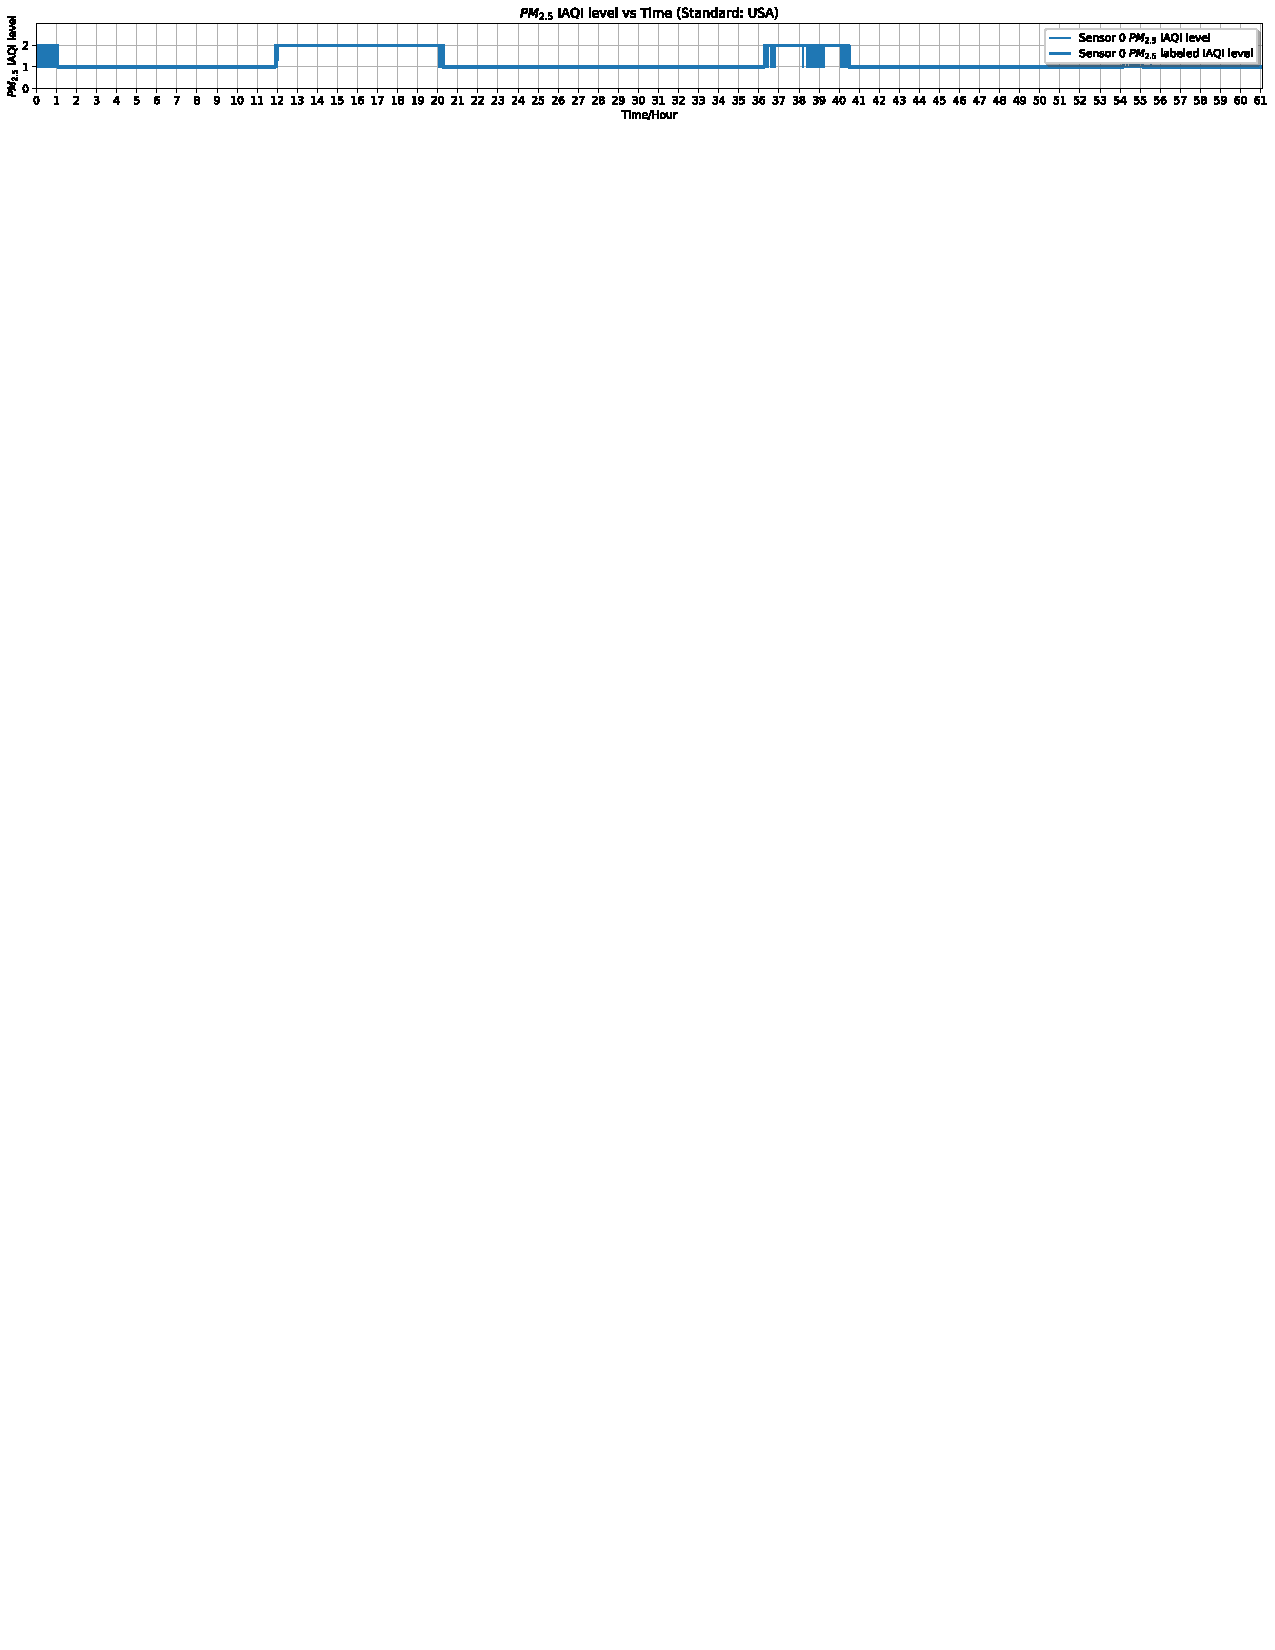
\includegraphics[width=\linewidth]{fig/labeled_iaqi_level/origin_and_labeled/pm25_0.png}
    \caption{Sensor 0's $PM_{2.5}$ origin and labeled IAQI level.}
    \label{fig:pm25_0_origin_and_labeled_level}
\end{figure}

\subsection{Data Polygonization}

To make use of the time elapse information, we did the same modeling as in \cite{rouet2017machine}. We did a similar transformation for the IAQI level plots (after labeling). Between two change points of the IAQI level, we transferred the level step-ups and downs into increasing and decreasing lines following the formula below:

\begin{equation}
    Level_t = (Level_{end}-Level_{begin}) / t-t_{begin}
\end{equation}

Dash lines in Figure \ref{fig:pm25_0_labeled_level} shows the results. These triangular lines will be label data for our later supervised learning regression problem.

\begin{figure}
    \centering
    \includegraphics[width=\linewidth]{fig/labeled_iaqi_level/pm25_0_labeled_iaqi_level.png}
    \caption{Sensor 0's labeled $PM_{2.5}$ IAQI level and its polygonization.}
    \label{fig:pm25_0_labeled_level}
\end{figure}

As the same with the modeling for acoustic data in \cite{rouet2017machine}, transferring step functions into linearly increasing/decreasing lines is a very useful method for preparing supervising data. These data contain linear time information. Thus the model can learn time variance knowledge between two change points of the IAQI level.

The level polygonal lines w.r.t. their manually labeled level curves can be written as equations with the form below:

\begin{equation}
    \label{formula:polygonal}
    L_i(t)=k_i*t+b_i, where t\in[t_i,t_{i+1}]
\end{equation}

Where $k_i$ is the slope of the curve, $t_i$ and $t_{i+1}$ start and end time point for every interval of the polygonal line. When $k_i>0$, the trend of the IAQI level is rising, and vice versa. The absolute value of $k_i$ is the approximate and potential changing speed of the IAQI level.

Thus, every polygonal line can be divided into several segments within time interval $t_i$ to $t_{i+1}$, and every segment estimates the 1-order approximate trend w.r.t. original IAQI level within the corresponding time interval. For the i-th segment, $k_i$ is $k_i =\frac{l_{i+1}-l_i}{t_{i+1}-t_i}$, where $l_{i+1}$ and $l_i$ are the original IAQI levels at end time $t_{i+1}$ and start time and $t_i$.

Finally, similar to B. Rouet-Leduc's work on earthquake predicting \cite{rouet2017machine} where the time-to-failures curve acts as y label, our experiments will take these polygonized IAQI level lines as the supervising data.
